% Template for PLoS
% Version 3.8 Apr 2026
%
% % % % % % % % % % % % % % % % % % % % % %
%
% -- IMPORTANT NOTE
%
% This template contains comments intended 
% to minimize problems and delays during our production 
% process. Please follow the template instructions
% whenever possible.
%
% % % % % % % % % % % % % % % % % % % % % % % 
%
% Once your paper is accepted for publication, 
% PLEASE REMOVE ALL TRACKED CHANGES in this file 
% and leave only the final text of your manuscript. 
% PLOS recommends the use of latexdiff to track changes during review, as this will help to maintain a clean tex file.
% Visit https://www.ctan.org/pkg/latexdiff?lang=en for info.
%
%
% IMPORTANT
% Below are a few tips to help format manuscript according to our specifications. For more tips to help reduce the possibility of formatting errors during conversion, please see our LaTeX guidelines at http://journals.plos.org/plosone/s/latex
%
% There are no restrictions on package use within the LaTeX files except that no packages listed in the template may be deleted.
%
% Please do not include colors or graphics in the text.
%
% The manuscript LaTeX source should be contained within a single file (do not use \input, \externaldocument, or similar commands).
%
% % % % % % % % % % % % % % % % % % % % % % %
%
% -- FIGURES AND TABLES
%
% Please include tables/figure captions directly after the paragraph where they are first cited in the text.
%
% DO NOT INCLUDE GRAPHICS IN YOUR MANUSCRIPT
% - Figures should be uploaded separately from your manuscript file. 
% - Figures generated using LaTeX should be extracted and removed from the PDF before submission. 
% - Figures containing multiple panels/subfigures must be combined into one image file before submission.
% For figure citations, please use "Fig" instead of "Figure".
% See http://journals.plos.org/plosone/s/figures for PLOS figure guidelines.
%
% Tables should be cell-based and may not contain:
% - spacing/line breaks within cells to alter layout or alignment
% - do not nest tabular environments (no tabular environments within tabular environments)
% - no graphics or colored text (cell background color/shading OK)
% See http://journals.plos.org/plosone/s/tables for table guidelines.
%
% For tables that exceed the width of the text column, use the adjustwidth environment as illustrated in the example table in text below.
%
% % % % % % % % % % % % % % % % % % % % % % % %
%
% -- EQUATIONS, MATH SYMBOLS, OTHER SPECIAL FORMATTING
%
% - For bold symbols, use the \boldsymbol command and not \mathbf. 
% - For inline equations, please be sure to include all portions of an equation in the math environment.  For example, x$^2$ is incorrect; this should be formatted as $x^2$ (or $\mathrm{x}^2$ if the romanized font is desired).
% - Do not include text that is not math in the math environment. For example, CO2 should be written as CO\textsubscript{2} instead of CO$_2$.
% - Avoid capturing simple text as equations, for example $<$.
% - For inline equations, please do not include punctuation (commas, etc) within the math environment unless this is part of the equation.
% - When adding superscript or subscripts outside of brackets/braces, please group using {}.  For example, change "[U(D,E,\gamma)]^2" to "{[U(D,E,\gamma)]}^2". 
% - Do not use \cal for caligraphic font.  Instead, use \mathcal{}.
% - Avoid splitting for fragmenting a single equation into multiple objects/environments, for example $f(x)$ = $g(x)$ + $h(x)$.
% - Use math environment for all equations, do not mimic using text.
% - Avoid using single letters in math mode where possible.
% - Always use matching parentheses and delimiters, avoid mixing math and text brackets.
% - Insert spaces around inline equations to ensure proper display after conversion.
% - Do not use forced numbers for display equation labeling or suppress numbering with \nonumber. 
%
% % % % % % % % % % % % % % % % % % % % % % % % 
%
% Please contact customercare@plos.org with any questions.
%
% % % % % % % % % % % % % % % % % % % % % % % %

\documentclass[10pt,letterpaper]{article}
\usepackage[top=0.85in,left=2.75in,footskip=0.75in]{geometry}

% amsmath and amssymb packages, useful for mathematical formulas and symbols
\usepackage{amsmath,amssymb}

% Use adjustwidth environment to exceed column width (see example table in text)
\usepackage{changepage}

% textcomp package and marvosym package for additional characters
\usepackage{textcomp,marvosym}

% cite package, to clean up citations in the main text. Do not remove.
\usepackage{cite}

% Use nameref to cite supporting information files (see Supporting Information section for more info)
\usepackage{nameref,hyperref}

% line numbers
\usepackage[right]{lineno}

% ligatures disabled
\usepackage[nopatch=eqnum]{microtype}
%\DisableLigatures[f]{encoding = *, family = * }

% color can be used to apply background shading to table cells only
\usepackage[table]{xcolor}

% array package and thick rules for tables
\usepackage{array}

% create "+" rule type for thick vertical lines
\newcolumntype{+}{!{\vrule width 2pt}}

% create \thickcline for thick horizontal lines of variable length
\newlength\savedwidth
\newcommand\thickcline[1]{%
  \noalign{\global\savedwidth\arrayrulewidth\global\arrayrulewidth 2pt}%
  \cline{#1}%
  \noalign{\vskip\arrayrulewidth}%
  \noalign{\global\arrayrulewidth\savedwidth}%
}

% \thickhline command for thick horizontal lines that span the table
\newcommand\thickhline{\noalign{\global\savedwidth\arrayrulewidth\global\arrayrulewidth 2pt}%
\hline
\noalign{\global\arrayrulewidth\savedwidth}}


% Remove comment for double spacing
%\usepackage{setspace} 
%\doublespacing

% Text layout
\raggedright
\setlength{\parindent}{0.5cm}
\textwidth 5.25in
\textheight 8.75in

% Bold the 'Figure #' in the caption and separate it from the title/caption with a period
% Captions will be left justified
\usepackage[aboveskip=1pt,labelfont=bf,labelsep=period,justification=raggedright,singlelinecheck=off]{caption}
\renewcommand{\figurename}{Fig}

% Please use the included `plos2025.bst` as your BibTeX style
\bibliographystyle{plos2025}

% Remove brackets from numbering in List of References
\makeatletter
\renewcommand{\@biblabel}[1]{\quad#1.}
\makeatother




% Header and footer (from the PLOS template)
\usepackage{lastpage,fancyhdr,graphicx}
\usepackage{epstopdf}
\usepackage{booktabs}
\pagestyle{fancy}
\fancyhf{}
\rfoot{\thepage/\pageref{LastPage}}
\renewcommand{\headrulewidth}{0pt}
\renewcommand{\footrule}{\hrule height 2pt \vspace{2mm}}
\fancyheadoffset[L]{2.25in}
\fancyfootoffset[L]{2.25in}
\lfoot{\today}
\graphicspath{{figures/}}

\begin{document}
\vspace*{0.2in}

\begin{flushleft}
{\Large
\textbf{HOBench: a literature-based benchmark for hierarchical orthology inference, built by AI agents}
}
\newline
\\
{}[Authors to be added by the human maintainer]\textsuperscript{1}
\\
\bigskip
\textbf{1} {}[Affiliation]
\\
\bigskip
\end{flushleft}

\noindent\fbox{\parbox{0.95\linewidth}{\textbf{Note on how this work was produced.} This study was an experiment in
testing whether AI agents can run a bioinformatics research project. An AI agent acted as principal investigator (PI)
and directed AI subagents through the literature survey, design, data curation, software, analysis, this manuscript
and the accompanying repository. Humans wrote the prompts, supplied papers that the agents requested, and restarted
the session after usage limits. No human checked the curated data or the code line by line before this draft. The
agent setup is described in Methods; the prompts and the complete process record are in the repository.}}

\section*{Abstract}
Benchmarks for orthology inference mostly score pairwise orthology or flat orthologous groups. Hierarchical
orthologous groups (HOGs) state, for every taxonomic level, which genes descend from one ancestral gene.
Existing benchmarks score HOGs only through these flattened views. We built HOBench, a benchmark that scores HOGs against evolutionary
histories asserted in publications. HOBench contains five species panels (90 species from UniProt reference
proteomes) and 32 curated reference families and collections, including 1,976 yeast whole-genome duplication (WGD)
gene sets from the Yeast Gene Order Browser and 498 \textit{Xenopus laevis} homeolog pairs. Each reference is a tree
with speciation, duplication, transfer and unresolved nodes, in which literature events are placed on species-tree
branches, often as intervals. All four metrics derive from one quantity, the most recent level at which two genes
share a HOG: per-level group F1, merge-level accuracy, recovery of literature duplications and family-membership F1.
We report each next to trivial baselines. In one pooled test over 13 headline items, OrthoFinder 3 scored higher than
FastOMA on per-level F1 (+0.054; Holm-adjusted $p=0.035$); the other endpoints were not significant. Both tools
classified most yeast pseudo-orthologs (paralogs left by reciprocal gene loss) as orthologs. They failed on WGDs in
opposite ways: OrthoFinder merged ohnolog copies, FastOMA split each copy's orthologs. Gene fragmentation lowered
accuracy more than contamination, species-tree changes or taxon removal. The work was done by AI agents as a test of
agent-run research (see note above). The sample of families is small and several design choices are ours rather than
community standards, so the results should be read as a prototype. Code, references and tool outputs are available
for scoring new methods.

\section*{Author summary}
Genes in different species are related through speciation and gene duplication. Methods for orthology inference
reconstruct these relations, and many now output hierarchical groups: for each ancestor in a species tree, the genes
that descend from one ancestral gene. Existing benchmarks do not test whether these hierarchies are correct at each
level. We collected gene families whose evolutionary histories are described in the literature, encoded what the
papers assert (and only that), and wrote metrics that test the hierarchy level by level. We used the benchmark to
compare two widely used methods and found specific, repeatable failure modes, such as mistaking paralogs for
orthologs after whole-genome duplication. The project was carried out by AI agents under human-written prompts, as
an experiment in agent-run research. We describe what the agents did, which of their ideas failed, and which
limitations remain.

\linenumbers

\section*{Introduction}
Orthologs are genes that diverged by speciation; paralogs diverged by duplication. A hierarchical orthologous group
(HOG) at a taxonomic level $L$ is the set of genes that descend from a single gene in the last common ancestor of the
species below $L$~\cite{altenhoff2013hogs,train2017gethogs}. A set of HOGs at all levels is equivalent to a reconciled
gene tree in which duplications are placed on species-tree branches. Several current methods output HOGs, including
OrthoFinder~\cite{emms2019orthofinder,emms2026orthofinder3} and FastOMA~\cite{majidian2025fastoma}.

The Quest for Orthologs (QfO) benchmark service~\cite{altenhoff2016qfo,nevers2022qfo} evaluates predicted ortholog
pairs with tests based on species-tree discordance, reference gene trees and function. OrthoBench scores flat
orthogroups against 70 curated reference groups at one level, Bilateria~\cite{trachana2011orthobench,emms2020orthobench}.
SwissTree provides expert-curated reconciled gene trees~\cite{boeckmann2011swisstree}, but they are scored through
ortholog pairs. Simulated data allow exact HOG evaluation~\cite{altenhoff2013hogs,dalquen2012alf}, but they lack
real-data error sources such as annotation errors. A recent review notes that HOG-specific benchmarking is still
missing~\cite{sartonloheac2025hogs}. We found no real-data benchmark that scores HOGs level by level or checks
whether specific duplications described in the literature are recovered.

Building such a benchmark is mainly a problem of data collection. Many gene families have published phylogenies, but the
information is spread over text, tables, trees and supplements, uses outdated identifiers, and is often only partly
resolved. A useful reference must record exactly what each publication asserts and map it to current proteomes. Everything
else must stay unscored. It should also cover the phenomena that make orthology inference hard: whole-genome duplication
(WGD) with differential gene loss, horizontal gene transfer (HGT), deep paralogy, promiscuous domains, annotation
errors and contamination.

We present HOBench, a benchmark built by AI agents that addresses this problem for 32 families and collections in
five species panels. We describe the data collection, the reference encoding and the metrics, and we use the
benchmark to compare OrthoFinder and FastOMA. We also report the process: the whole project was an experiment in
whether AI agents can run a bioinformatics study, and several of its decisions and failures are informative for that
reason.

\section*{Results}

\subsection*{Overview of the benchmark}
HOBench has three parts (Fig~\ref{fig1}): species panels with proteomes and species trees, reference families curated
from publications, and metrics with controls. Table~\ref{tab1} lists the panels. We chose five panels instead of one
large species set because the phenomena of interest occur in different clades and because orthology inference on a
single 90-species set exceeded our compute budget (see Methods). Panels are yeasts (Y), prokaryotes (K), eukaryotes
with prokaryote outgroups (E), vertebrates (V) and plants (P). Each panel has a binary species tree whose internal
nodes are named levels; topologies come from published phylogenomic studies~\cite{shen2018yeast,coleman2021rooting,burki2020eukaryotes}.

\begin{figure}[!h]
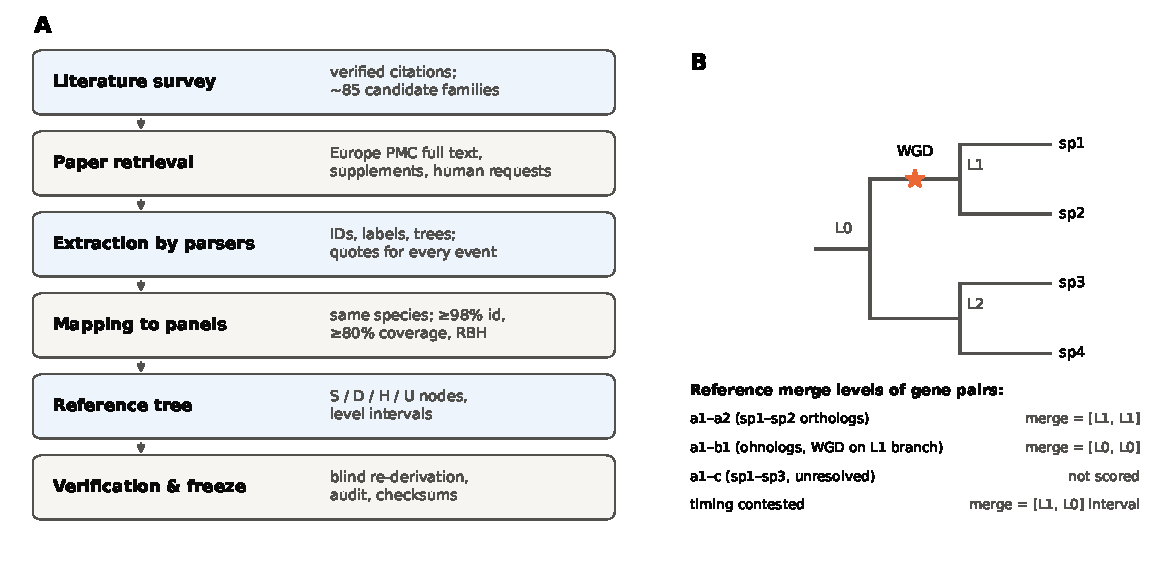
\includegraphics[width=\linewidth]{Fig1.pdf}
\caption{{\bf Data collection and the merge-level formalism.}
(A) Steps from literature to frozen reference families (details in Methods). (B) Toy example. Genes a1 and b1 are
ohnologs in species sp1 that arose from a WGD on the branch leading to level L1; a2 is the sp2 ortholog of a1. The
merge level of a gene pair in the reference is the most recent level at which the two genes descend from one ancestral gene:
L1 for the orthologs a1--a2 and L0 for the ohnologs a1--b1. Pairs that a source does not resolve are not scored.
Contested event timing gives an interval of allowed merge levels.}
\label{fig1}
\end{figure}

\begin{table}[!ht]
\begin{adjustwidth}{-2.25in}{0in}
\centering
\caption{{\bf Species panels.} Proteomes are UniProt reference proteomes, release 2026\_03~\cite{uniprot2025}, one
protein per gene. Subsets are described in Methods.}
\begin{tabular}{llrrrl}
\toprule
Panel & Scope & Species & Proteins & Scored on & Main events \\
\midrule
Y & Saccharomycetaceae + outgroups & 16 & 85,185 & full & allopolyploid WGD, gene loss, HGT \\
K & Bacteria and archaea & 21 & 68,128 & full & ancient paralogs, controls, decoys \\
E & Eukaryotes + 9 prokaryotes & 34 & 340,217 & 25,855 subset & pre-LECA paralogs \\
V & Vertebrates + 2 chordates & 17 & 447,758 & 70,000 subset & 2R, 3R, allotetraploidy \\
P & Green plants & 14 & 417,784 & 25,429 subset & plant WGDs, HGT, nested families \\
\bottomrule
\end{tabular}
\label{tab1}
\end{adjustwidth}
\end{table}

\subsection*{Reference families from the literature}
Agents screened about 85 candidate families described in the literature and kept those with machine-readable member
lists (supplementary tables, labelled trees or curated databases) and at least four panel species after mapping. They
excluded sources whose orthology assignments come from tools for orthology inference (OMA, OrthoFinder, Ensembl Compara and
names projected from it, PANTHER, TreeFam, eggNOG, OrthoDB, PLAZA, OHNOLOGS), because using them as truth would favour
the tools they come from. The final catalogue has 32 entries (Table~\ref{tab2}; full list in S1 Table): 13 headline
items, 3 control families, 10 non-homologous decoy families, and 6 secondary families that missed the mapping or
verification thresholds. Together they contain about 31,800 genes, 85 duplications asserted in the text (tier T1) and
2,138 duplications derived from curated classifications (tier T2).

\begin{table}[!ht]
\begin{adjustwidth}{-2.25in}{0in}
\centering
\caption{{\bf Headline reference families and controls.} Members = genes mapped to the panel proteomes. Collections are scored as one item each.}
\begin{tabular}{lllrrl}
\toprule
ID & Family & Source & Members & Species & Phenomena \\
\midrule
Y01 & YGOB pillars (1,976 units) & \cite{byrne2005ygob,scannell2007,marcethouben2015} & 26,166 & 13 & WGD, loss, hidden paralogy \\
Y03 & URA1 dihydroorotate dehydrogenase & \cite{hall2005ura1,gojkovic2004} & 16 & 14 & HGT from bacteria \\
E01 & Kinesins & \cite{wickstead2010kinesin} & 399 & 19 & pre-LECA paralogs, motor domain \\
E02 & ARF/Arl/Sar GTPases & \cite{vargova2021arf} & 325 & 22 & pre-LECA paralogs, short domain \\
E03 & Rab GTPases & \cite{klopper2012rab} & 388 & 15 & pre-LECA paralogs \\
E04 & Tubulins & \cite{findeisen2014tubulin} & 170 & 24 & pre-LECA paralogs \\
E07c & Adaptor complex scaffolds & \cite{hirst2014tset} & 35 & 14 & pre-LECA paralogs \\
V02 & Visual opsins & \cite{lagman2013opsins} & 41 & 8 & 2R, 3R \\
V03 & Hox clusters & \cite{holland2007homeobox,session2016xenopus} & 237 & 5 & tandem, 2R, 3R \\
V07 & \textit{X. laevis} L/S homeologs (498 units) & \cite{session2016xenopus} & 1,494 & 2 & allotetraploidy \\
P02 & bHLH transcription factors & \cite{pires2010bhlh} & 435 & 5 & short domain, plant WGDs \\
P03 & GID1 within carboxylesterases & \cite{yoshida2018gid1} & 94 & 9 & nested family \\
P04 & Major intrinsic proteins & \cite{danielson2008mips} & 119 & 4 & HGT (NIPs), plant WGDs \\
\midrule
K01 & Ribosomal proteins (40 units; control) & \cite{yutin2012rprot,galperin2021cog} & 651 & 19 & single copy \\
K02 & EF-Tu/EF-G (control) & \cite{baldauf1996,iwabe1989} & 47 & 19 & pre-LUCA paralogs \\
E05 & MCM2--9 (control) & \cite{liu2009mcm} & 113 & 18 & pre-LECA paralogs \\
K04 & Analogous enzymes (5 pairs; decoys) & \cite{omelchenko2010} & 108 & 5--14 & must never merge \\
\bottomrule
\end{tabular}
\label{tab2}
\end{adjustwidth}
\end{table}

\paragraph{Conceptual approach.} A reference family records only what its sources assert. Each family is a rooted
tree whose leaves are UniProt accessions and whose internal nodes are speciation (S), duplication (D), HGT acquisition
(H) or unresolved (U). Duplications are placed on a species-tree branch, or on an interval of branches when the
timing is uncertain or contested. Pairs whose lowest common node is U are not scored. This design addresses the main
weakness of literature benchmarks: absence of a statement is not evidence. It also allows partial references, which
most families are.

Several histories needed explicit intervals. The yeast WGD probably arose by hybridization of two lineages
~\cite{marcethouben2015}, so ohnolog copies may coalesce at the ancestor of the post-WGD and ZT clades or as deep as
the Saccharomycetaceae root; we encoded that range. YGOB synteny tracks~\cite{byrne2005ygob} show which single-copy
genes in two post-WGD species are paralogs after reciprocal loss (pseudo-orthologs~\cite{scannell2006}); we scored
these as paralogs. \textit{X. laevis} L and S homeologs~\cite{session2016xenopus} are a duplication on the
\textit{X. laevis} branch. HGT was encoded so that the transferred copy and native copies are never in one HOG within
the recipient lineage.

\paragraph{Technical approach.} Agents retrieved open-access full texts and supplements from Europe PMC, extracted
identifiers and labels with committed per-family parser scripts (no identifiers were typed by hand), mapped them to
the panel proteomes and compiled the reference tree. Mapping used UniProt identifier mapping or same-species sequence
matches ($\geq$98\% identity, $\geq$80\% coverage of both sequences, reciprocal best hit). Every label, event level
and tag carries a source locator and a verbatim quote, which a script checks against the stored source text. A
different agent re-derived up to 30 sampled assertions per family without seeing the claimed values; 22 of 23
verification groups passed (at most 1 discrepancy) and one (globins) failed and was moved to the secondary set
(S2 Text). Families in which fewer than 80\% of members mapped uniquely were also kept out of the headline set. We froze the
references by checksum before scoring the larger panels. Later corrections are logged with values before and after
the change.

\subsection*{Metrics}
For two genes $a$ and $b$, the \emph{merge level} $m(a,b)$ is the most recent level at which they belong to the same
HOG. Orthologs merge at the last common ancestor of their species; paralogs merge above the duplication. The reference
gives an interval $[m_{lo}, m_{hi}]$ for each asserted pair; a predicted merge level is correct if it lies inside. The
merge-level matrix of a reconciled tree is a symbolic ultrametric~\cite{hellmuth2013cograph,lafond2014orthology},
This is why per-level HOG partitions, pairwise relations and duplication timing can all be read from the same matrix. We defined
four primary endpoints before scoring the larger panels:
\begin{enumerate}
\item \textbf{Per-level B-cubed F1}~\cite{amigo2009bcubed}: agreement between predicted and reference HOGs at each
level, computed per gene and averaged over levels.
\item \textbf{Merge-level accuracy}: for each asserted reference node, the fraction of its gene pairs with a correct
predicted merge level, averaged over nodes so that large subfamilies do not dominate.
\item \textbf{Event recovery}: a literature duplication is recovered if its copies are in different HOGs at the event
level and at least half of each copy's reference orthologs share a HOG. Requiring both sides prevents trivial
predictions from scoring.
\item \textbf{Family-membership F1}: precision and recall of family membership, computed only where errors are
defined: in species for which a source states a genome-wide search, against declared decoys, and for separations that
the reference asserts.
\end{enumerate}
Secondary measures include the OrthoBench family measures~\cite{emms2020orthobench}, signed level errors (too old or
too young), contamination by decoys, and a skill score $(s-b)/(1-b)$ relative to the best trivial baseline $b$. The
baselines are all-singletons, one big HOG per family, and random relabelling. We report no composite score.

\paragraph{Validation of the metrics.} The test suite has 95 tests with hand-derived expected values. Ten deliberate
code mutations (for example, swapping speciation and duplication handling) all made the suite fail. On every family,
the reference-derived prediction scored 1.0 on all endpoints. Running trivial baselines on real data exposed five
metric defects that toy data had not shown (S2 Text). For example, all-singletons first "recovered" 86\% of YGOB WGD
events, because the hybrid-origin interval has no upper bound within the family's range and many copies are single
genes. We therefore score only events that both baselines can fail. Of 1,592 YGOB WGD events, 202 are testable.

\subsection*{Tool comparison}
We ran OrthoFinder 3.1.5 (default and DendroBLAST modes) and FastOMA 0.5.0. Both tools received the same proteomes and species trees.
Fig~\ref{fig2} shows the primary endpoints per panel with the best trivial baseline. Per-panel results are descriptive
because each panel has two to five headline items. In the pooled confirmatory test (paired permutation, OrthoFinder
default versus FastOMA, Holm correction over the four endpoints~\cite{holm1979}; Table~\ref{tab3}), OrthoFinder scored
higher on per-level F1. Differences in the other endpoints pointed the same way but were not significant. Most of the
difference came from panels E and V. OrthoFinder in DendroBLAST mode had the highest pooled merge-level accuracy
(0.886 versus 0.846 for default OrthoFinder and 0.712 for FastOMA; $n=13$) and event recovery (0.617, 0.479 and 0.194;
$n=11$), but not on every panel.

\begin{figure}[!h]
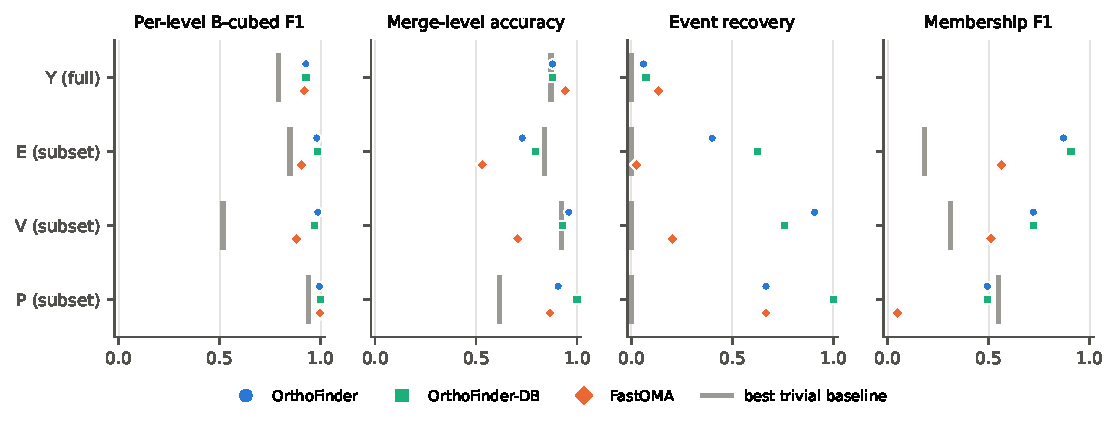
\includegraphics[width=\linewidth]{Fig2.pdf}
\caption{{\bf Primary endpoints per panel.} Mean over headline items (a collection counts as one item); grey bars show
the best trivial baseline. OrthoFinder-DB = OrthoFinder DendroBLAST mode. Number of items per panel: Y 2, E 5 (membership
3), V 3 (events 2, membership 1), P 3 (events 2, membership 1). Panel K has no headline item with asserted pairs.
Membership F1 is undefined for Y.}
\label{fig2}
\end{figure}

\begin{table}[!ht]
\centering
\caption{{\bf Confirmatory comparison, OrthoFinder minus FastOMA.} Paired permutation test over pooled headline items
(10,000 sign flips), Holm-adjusted over the four endpoints. Panels Y and K in full mode, E, V and P in subset mode.}
\begin{tabular}{lrrr}
\toprule
Endpoint & Items & Mean difference & Holm $p$ \\
\midrule
Per-level B-cubed F1 & 13 & +0.054 & 0.035 \\
Merge-level accuracy & 13 & +0.134 & 0.058 \\
Event recovery & 11 & +0.285 & 0.12 \\
Membership F1 & 5 & +0.315 & 0.12 \\
\bottomrule
\end{tabular}
\label{tab3}
\end{table}

Trivial baselines put the numbers in context. On panel E, one big HOG per family had higher merge-level accuracy
(0.838) than both tools (OrthoFinder 0.729, FastOMA 0.531). Most asserted nodes there are speciation nodes, and both
tools split speciation pairs (FastOMA 66.7\% and OrthoFinder 20.4\% of such pairs). FastOMA also merged 24.4\% of pairs
under duplication nodes too early, mostly at the eukaryote level (OrthoFinder 0.1\%). On plant bHLH proteins, FastOMA
had high membership precision (0.959) but recall of 0.025: it spread the 435 members over 186 groups.

\subsection*{Phenomena that separate the methods}
\textbf{Hidden paralogy after WGD.} In 49 YGOB units, \textit{S. cerevisiae} and \textit{C. glabrata} each kept a
single copy, but from different WGD tracks. These genes look like orthologs but are paralogs~\cite{scannell2006}.
OrthoFinder classified 4\% of these pairs correctly and FastOMA 12\%, compared with 91\% and 87\% for 1,189 true
ortholog pairs (Fig~\ref{fig3}A).

\textbf{WGD events.} Over the 201 testable YGOB WGD events, the two tools failed in opposite ways (Fig~\ref{fig3}B).
OrthoFinder kept ohnolog copies apart in only 26\% of events but kept each copy's orthologs together in 79\%. FastOMA
kept copies apart in 64\% but kept each copy together in only 57\%. Within YGOB units, accuracy at WGD nodes was lower
than at speciation nodes by 0.68 for OrthoFinder and 0.21 for FastOMA ($n=532$ units). The direction of OrthoFinder's
error agrees with the known tendency of reconciliation to misplace duplications when gene trees are
uncertain~\cite{hahn2007bias}, but we did not test the cause.

\textbf{Vertebrate duplications.} FastOMA recovered 8\% of the 13 Hox 2R events and 9\% of the 11 3R events;
OrthoFinder recovered 77\% and 82\% (Fig~\ref{fig3}C). FastOMA placed \textit{X. laevis} L/S homeologs correctly in
43\% of 333 units and split 56\% of them; OrthoFinder placed 99\% correctly.

\begin{figure}[!h]
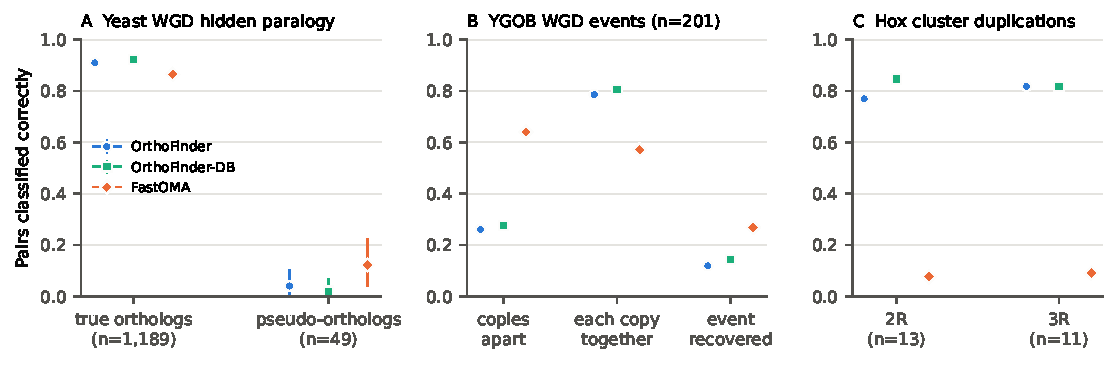
\includegraphics[width=\linewidth]{Fig3.pdf}
\caption{{\bf Phenomena.} (A) Fraction of yeast gene pairs classified correctly, for true orthologs (same YGOB track)
and pseudo-orthologs (single surviving copies on different tracks); 95\% bootstrap intervals. (B) Testable YGOB WGD
events: fraction with copies in different HOGs at the event level, minimum fraction of each copy's orthologs that
share a HOG, and events recovered. (C) Recovery of Hox cluster duplications at the 2R (Gnathostomata) and 3R
(Teleostei) levels.}
\label{fig3}
\end{figure}

\subsection*{Robustness to data errors}
We perturbed the yeast panel and re-ran both tools (Fig~\ref{fig4}). Splitting 10\% of family members into two
fragments lowered merge-level accuracy by 0.050 (OrthoFinder) and 0.114 (FastOMA) when both fragments had to be
placed correctly. When one correctly placed fragment was enough, the drops were 0.003 and 0.024. Inserting 20 or 200
human proteins into the \textit{K. lactis} proteome, swapping one contested species-tree node, or removing two pre-WGD
species changed the primary endpoints by at most 0.005. In the 200-protein test, both tools placed about half of the
contaminants into HOGs with yeast reference genes, but the relations among the yeast genes did not change. A repeated
OrthoFinder run was identical to the first; a repeated FastOMA run differed in 2\% of YGOB units (mean change in
merge-level accuracy $-0.001$, SD 0.038). FastOMA's small deltas are therefore within its run-to-run noise. These
perturbations were mild, so they show that the tools are not sensitive to them at this strength, not that they are
robust in general.

\begin{figure}[!h]
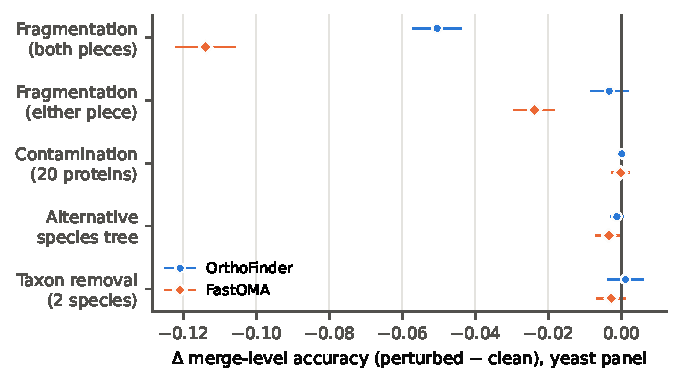
\includegraphics[width=0.75\linewidth]{Fig4.pdf}
\caption{{\bf Effect of perturbations on the yeast panel.} Change in merge-level accuracy (perturbed minus clean;
95\% bootstrap interval over 1,977 units). Fragmentation is scored with two rules: the parent gene counts as correct if
both fragments, or either fragment, are placed correctly. The 200-protein contamination test (not shown) gave changes
of $+0.0004$ (OrthoFinder) and $-0.0010$ (FastOMA).}
\label{fig4}
\end{figure}

\subsection*{Scoring on proteome subsets}
Full runs on panels E, V and P would have taken several hours per tool, so we scored them on subsets: all proteins
with DIAMOND hits~\cite{buchfink2021diamond} to frozen reference members, a capped sample of domain-only hits, and a
random background. We tested this choice on panels Y and K, where we ran both modes. For all tools and testable primary
endpoints, the subset-minus-full difference was within the pre-registered margin of $\pm0.05$ (TOST, 90\% paired
interval~\cite{schuirmann1987tost}), and 96--99.6\% of gene pairs had the same predicted merge level. The test was
informative mainly on K (subset 6\% of the proteome); on Y the subset covered 54\% of the proteome. Results for E, V
and P are therefore conditional on subset mode.

\section*{Discussion}
HOBench shows that literature-based references can test hierarchical orthology at specific levels and for specific
events, and that such tests separate methods in ways that pairwise benchmarks do not show. The hidden-paralogy result
is the clearest example: both tools score well on true yeast orthologs and poorly on pseudo-orthologs. A pairwise
benchmark that pools these pairs would show a single high number.

The benchmark has clear limits. First, the number of independent families is small: 13 headline items, with two to
five per panel. Only the pooled test is inferential, and its power is low. Second, references are incomplete by
design. Many families are partly unresolved, and membership F1 is defined for only five items. Third, the families
are biased toward well-studied groups with machine-readable data. No headline family covers incomplete lineage sorting,
gene fusion or a fast-evolving lineage, and HGT has one headline family. Fourth, some choices are ours and debatable:
the interval for the yeast WGD, together with copies that consist of a single gene, makes 87\% of YGOB events
untestable, the Hox reference relies on curated nomenclature,
and two prokaryote families locate proteins through COG membership~\cite{galperin2021cog}. Fifth, FastOMA assigns
proteins with OMAmer~\cite{rossier2021omamer}, whose database is built from OMA HOGs that may include our species; we
could not remove this possible advantage within the budget. Sixth, we compared two tools in two OrthoFinder modes;
agreement analyses with more methods would be more informative. Seventh, panels E, V and P were scored in subset mode,
which we validated only on Y and K.

\paragraph{What the agent experiment showed.} The agents completed the survey, curation, software and analysis in
about 21 hours of wall-clock time, of which about 11 hours were lost when the account reached its usage limit three times. The most
useful process elements were independent design reviews, which found real defects before scoring, mechanical checks
of provenance, and trivial baselines run on real data, which exposed five metric defects. The main failures were
launching too many subagents at once (which triggered the first outage), late checks of data sources (a tool-derived
table was found only during curation), and accepting metric definitions before running controls. An independent
agent fact-checked the first report against the result files and found eight wrong numbers and several overstatements,
which we corrected. Because no human reviewed the curated references line by line, errors may remain; the blind
re-derivation bounds the error rate per family only roughly (at most 1 of 30 items wrong for passing families). S1 Text lists the main
ideas that did not work.

\section*{Methods}

\subsection*{Agent setup}
The project ran in Claude Code, an agent harness, on one compute node (12 cores, about 50 GB usable memory, no job
scheduler) with internet access. A PI agent received the project prompt and a goal message (both in the repository,
\texttt{prompts/}) and ran autonomously for 24 hours. It used Anthropic Claude models: a larger model for the PI, the
literature survey, core software, curation, design review and analysis, and a smaller, faster model for routine
engineering, verification, audits and fact-checking. The PI agent wrote the research record
(\texttt{RESEARCH\_TREE.md}, decisions D0--D12), process rules (\texttt{LESSONS.md}) and the design document, and it
launched 31 subagents: 4 literature surveyors, 4 software engineers (metrics, curation tools, provenance checks, tool
wrapper), 1 panel
and data engineer, 10 curators (two to six families each), 1 evaluator, 1 analyst, 1 blind verifier, 1 mutation tester,
1 catalogue builder, 1 release engineer, 1 design-review coordinator (which launched 7 reviewers), 2 second-round
reviewers, 2 process reviewers and 1 fact-checker. Subagents received written briefs and shared files through the project directory and git. They returned short
summaries, and the PI read these summaries rather than raw logs. Subagents could not see
each other's work unless it was committed. Reviewers and verifiers did not see the work they checked until they had
written their own assessments.

Humans intervened in three ways: they wrote the prompts, they supplied 49 of 50 paywalled papers or supplements that the
agents listed in a ranked request file, and after outages they typed "Try again" or "Please continue after stop". This
manuscript and the repository were written by the same PI agent after a second prompt (in the repository).

\subsection*{Literature and data survey}
Four subagents surveyed (i) orthology benchmarks and metrics, (ii) candidate families in animals and fungi, (iii)
candidate families in plants, protists and prokaryotes, and (iv) proteome sources, species panels and species trees.
They verified every citation against Europe PMC or Crossref and opened supplements to confirm that member lists
existed. The surveys produced 85 candidate families with phenomenon tags and data readiness, and a ranked list of 50
papers that could not be retrieved automatically.

\subsection*{Design and review}
The PI wrote a design document, which seven independent reviewer agents (external PI, prior work, statistics, data,
algorithms and compute, AI-agent failure modes, molecular evolution) reviewed. A coordinator merged their proposals.
The PI accepted the synthesis, which changed the merge levels in the reference from points to intervals, introduced two-sided
event recovery and membership F1, replaced an incorrect decoy set ($\beta$-lactamase classes A, C and D are
homologous) with non-homologous isofunctional enzymes~\cite{omelchenko2010}, and added mechanical provenance checks.
A second round (two reviewers) reviewed the design together with first results. Table~\ref{tab4} lists the main
decisions.

\begin{table}[!ht]
\begin{adjustwidth}{-2.25in}{0in}
\centering
\caption{{\bf Main design decisions.}}
\small
\begin{tabular}{p{5.2cm}p{6.0cm}p{5.6cm}}
\toprule
Decision & Reason & Consequence \\
\midrule
Score only asserted relations; unresolved = U & absence of a statement is not evidence & partial references are usable; fewer scored pairs \\
Merge levels in the reference as intervals & contested timing, allopolyploidy, HGT & correct WGD predictions were mis-scored with point values \\
Tool-derived sources excluded & avoid circularity & Braasch 2016 3R ohnologs dropped (Ensembl Compara) \\
Members extracted by parsers; quotes checked by script & prevent invented identifiers & slower curation \\
Same-species mapping, $\geq$98\% identity; $\geq$80\% mapped for headline & wrong paralog or homeolog otherwise & 6 families secondary \\
Allopolyploid interval for the yeast WGD & hybrid origin~\cite{marcethouben2015} & 87\% of YGOB events untestable \\
Score only testable events (both baselines can fail) & trivial predictors scored 0.86 & 202 of 1,592 YGOB events scored \\
Leaf-level duplications reported separately & one big HOG recovers them correctly & headline events = internal branches \\
Five panels; full mode for Y, K; subsets for E, V, P & compute budget & subset validated on Y, K only \\
Freeze references before scoring large panels & avoid tuning to results & corrections logged as errata \\
One pooled confirmatory test; panels descriptive & 2--5 items per panel & low power \\
\bottomrule
\end{tabular}
\label{tab4}
\end{adjustwidth}
\end{table}

\subsection*{Species panels}
Proteomes are UniProt reference proteomes, release 2026\_03~\cite{uniprot2025}, taken as one canonical protein per gene
from the UniProt FTP site and pinned by sha256. Panel species were chosen to cover each panel's events and to overlap
with species sampled in the source papers. Species trees were taken from published phylogenomic studies, made binary
and given level names; contested nodes are documented with citations in \texttt{panels/<P>/levels.tsv}, and each panel
has one alternative topology.

\subsection*{Curation protocol}
Curators followed a written protocol (repository, \texttt{docs/CURATION\_PROTOCOL.md}). They could not open tool
outputs. Each family has a \texttt{build.py} that reads stored source files and writes the member table, reference
tree, mapping report and assertion table. Assertions have three tiers: T1, stated in the text; T2, derived from curated
labels by fixed rules; T3, read from published trees with support $\geq$70\% bootstrap or $\geq$0.95 posterior. Headline
numbers use T1 and T2. The rule that genes with the same label and at most one gene per species are orthologs (an S
node) was not applied across WGD lineages unless the set was synteny-based, because reciprocal loss creates
pseudo-orthologs. When a source gave only a domain sequence (kinesin and myosin motor domains), mapping required a
domain of $\geq$250 residues covered to $\geq$90\% at $\geq$98\% identity. A script checked that each quote occurs in
the stored source, that each gene is in the pinned proteome, and that thresholds hold. A blind verifier re-derived
min(all, 30) seeded assertions per family from the source; two or more discrepancies failed the family (Clopper--Pearson
bounds reported~\cite{clopper1934}). A script searched all family files for tool-derived sources and references to tool
outputs and found none after review of flagged lines.

\subsection*{Tool runs}
A Python wrapper ran OrthoFinder 3.1.5 (\texttt{-s} with the panel tree; default and \texttt{-M dendroblast}) and the
FastOMA 0.5.0 Nextflow workflow with the same tree and precomputed OMAmer placements (LUCA database) and recorded
commands, versions, input checksums and run times. A flat baseline used OrthoFinder orthogroups without hierarchy. In
OrthoXML, levels were matched to panel levels by species content, and duplications were placed at the level declared
by the enclosing group (a later-placement reading was a sensitivity analysis, following pyHam~\cite{train2019pyham}).
Subsets were built once with DIAMOND (\texttt{--more-sensitive}, E $\leq10^{-5}$) from frozen member lists and stored
as identifier lists.

\subsection*{Statistics}
The unit of analysis is a family; a collection counts as one item, with its units aggregated first. Per-panel results
are descriptive. The confirmatory test is a paired sign-flip permutation test (10,000 permutations, fixed seed) per
primary endpoint over pooled headline items, with Holm correction~\cite{holm1979}. Agreement between methods uses
adjusted mutual information~\cite{vinh2010ami}. Robustness intervals are bootstrap intervals over units. The
subset-versus-full test is a two one-sided tests procedure with a margin of 0.05 fixed before the runs.

\subsection*{Ideas taken from the literature}
The HOG definition and its equivalence to reconciled trees come from OMA work~\cite{altenhoff2013hogs,train2017gethogs};
level induction in OrthoXML from pyHam~\cite{train2019pyham}; family-level fission and fusion measures from
OrthoBench~\cite{trachana2011orthobench,emms2020orthobench}; the use of expert reconciled trees as references from
SwissTree~\cite{boeckmann2011swisstree}; the benchmark-service framing from QfO~\cite{altenhoff2016qfo,nevers2022qfo};
the theory of orthology relations from~\cite{hellmuth2013cograph,lafond2014orthology}; hidden paralogy and synteny
tracks from~\cite{byrne2005ygob,scannell2006,scannell2007}; the hybrid WGD model from~\cite{marcethouben2015};
analogous enzymes as merge decoys from~\cite{omelchenko2010}; B-cubed, adjusted mutual information, TOST, Holm and
Clopper--Pearson methods from~\cite{amigo2009bcubed,vinh2010ami,schuirmann1987tost,holm1979,clopper1934}. Each reference
family uses the classifications and phylogenies of the papers cited in Table~\ref{tab2} and in its \texttt{family.yaml}.

\subsection*{Data and code availability}
The repository contains the \texttt{hobench} package, scripts to score a new method (\texttt{score\_method.py}),
frozen references with provenance, panel definitions, subset identifier lists, the outputs of all runs reported here,
result tables, the prompts and the complete process record. The proteomes used are provided as a release archive
(UniProt, CC BY 4.0). [Repository URL and archive DOI to be added by the maintainer.]

\section*{Supporting information}

\paragraph*{S1 Text.}
\label{S1_Text}
\textbf{Ideas that did not work.} Major approaches that the agents tried and abandoned or corrected, with reasons.

\paragraph*{S2 Text.}
\label{S2_Text}
\textbf{Metric errata and verification.} The five metric defects found by controls, the post-freeze reference
corrections, and blind-verification results per family (repository files \texttt{results/ERRATA.md},
\texttt{families/ERRATA.md}, \texttt{families/VERIFICATION.md}).

\paragraph*{S1 Table.}
\label{S1_Table}
\textbf{Catalogue of all 32 reference families and collections} with sources, mapping rates, events by tier,
verification status and abandoned candidates (repository \texttt{results/catalogue/}).

\section*{Acknowledgments}
We thank the authors of the cited studies, whose published classifications and phylogenies form the references.

\nolinenumbers

\bibliography{references}

\end{document}
